\section{能量极小}
\label{sec:ellip-energy}

一根绷紧的弦受到载荷后停在某个形状，这个形状是所有可能形状中总势能最小的。Poisson方程的弱解是否也是某种能量的极小点？第~\ref{sec:ellip-wellposed}节的三种弱形式都能这样解释吗？

\paragraph{能量泛函}
对$H$上的双线性型$a$和右端泛函$\ell$，定义二次泛函
\begin{equation}
 J(v)=\frac12a(v,v)-\ell(v).
 \label{eq:ellip-energy}
\end{equation}
对Dirichlet问题，$a$和$\ell$分别是式~\eqref{eq:ellip-bilinear}与$\int_\Omega fv$，所以
\[
 J(v)=\frac12\int_\Omega\bm{A}\nabla v\cdot\nabla v\,\mathrm{d}\bm{x}-\int_\Omega fv\,\mathrm{d}\bm{x} .
\]
第一项是梯度的储能，第二项是载荷做功的相反数，两者折中，形成平衡。

有限维的类比是对称正定的$\bm{K}$和二次函数$\frac12\bm{c}^\top\bm{K}\bm{c}-\bm{b}^\top\bm{c}$，令梯度为零，正是$\bm{K}\bm{c}=\bm{b}$。下面的定理是这件事的无限维版本。泛函的方向导数与极小点的一般理论可参考\BookChapterRef{chap:functional-optimization-variation}{卷五第29章“泛函优化”}，这里的二次泛函可以直接展开，不需要一般理论。

\begin{theorem}[弱解是能量的唯一极小点]
\label{thm:ellip-energy}
设$H$是实Hilbert空间，$a$是$H$上有界、强制且对称的双线性型，$\ell\in H^*$。对$u\in H$，下面两条等价：
\begin{enumerate}
 \item $a(u,v)=\ell(v)$对所有$v\in H$成立；
 \item $u$是$J$在$H$上的极小点。
\end{enumerate}
极小点存在且唯一，并且对所有$w\in H$，
\begin{equation}
 J(u+w)-J(u)=\frac12a(w,w).
 \label{eq:ellip-energy-gap}
\end{equation}
\end{theorem}

\begin{proof}
对任意$u,w\in H$，由双线性与对称性展开，
\[
 J(u+w)=J(u)+\bigl(a(u,w)-\ell(w)\bigr)+\frac12a(w,w).
\]

设第1条成立，括号为零，就得到式~\eqref{eq:ellip-energy-gap}。由强制性，$w\neq0$时$a(w,w)>0$，所以$u$是唯一的极小点。

设第2条成立。任取$v\in H$和实数$t$，取$w=tv$，极小性给出
\[
 0\leq J(u+tv)-J(u)=t\bigl(a(u,v)-\ell(v)\bigr)+\frac{t^2}2a(v,v).
\]
右端是$t$的二次函数，在$t=0$处取最小值$0$，所以一次项系数为零，即第1条成立。

极小点的存在由定理~\ref{thm:ellip-lax-milgram}给出。
\end{proof}

式~\eqref{eq:ellip-energy-gap}比“极小”的说法更强：任何候选的能量超出最优能量的部分，恰好是它到解的距离在能量范数下的平方的一半。

对称情形下，存在性也可以不用Lax--Milgram定理。此时$a(\cdot,\cdot)$本身是$H$上的一个等价内积，Riesz表示定理直接给出解；或者取极小化序列用平行四边形恒等式证明它是Cauchy列。这是对称问题的简化，非对称问题走不通。

\paragraph{手算比较}
继续用$-u''=1$，$u(0)=u(1)=0$，这时$J(v)=\frac12\int_0^1v'^2-\int_0^1v$。把真解$u_*=x(1-x)/2$代入：
\[
 J(u_*)=\frac12\cdot\frac1{12}-\frac1{12}=-\frac1{24}\approx-0.04167 .
\]

取几个其他的候选比较，都先把幅度调到各自的最优值。形如$cx(1-x)$的候选有
\[
 J=\frac{c^2}6-\frac c6,
\]
它在$c=1/2$处最小，正好回到真解。帐篷函数$s\min(x,1-x)$有$J=s^2/2-s/4$，最优幅度$s=1/4$给出$J=-1/32\approx-0.03125$。单个正弦$c\sin(\pi x)$的最优幅度是$c=4/\pi^3$，给出$J=-4/\pi^4\approx-0.04106$。

\begin{BookInlineFigure}
  \centering
  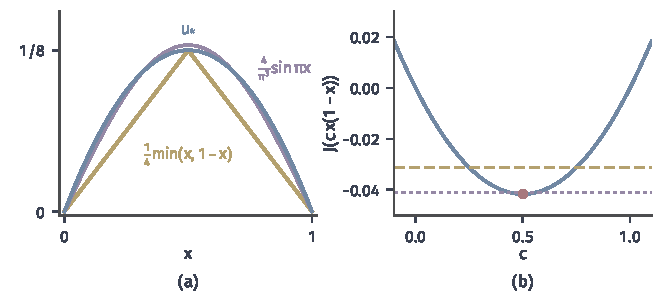
\includegraphics[width=112mm]{figures/06-differential-equations/02-partial-differential-equations/matplotlib/ellip-energy-competition/figure.pdf}
  \caption{能量比较，$f=1$，零边界。(a)真解$u_*$（蓝）与两个候选：帐篷（黄）和单个正弦（紫）。(b)蓝线是$J(cx(1-x))$，红点是$c=1/2$处的最小值$-1/24$；黄色虚线和紫色点线分别是帐篷和正弦的能量，都高于$-1/24$。}
  \label{fig:ellip-energy-competition}
\end{BookInlineFigure}

图~\ref{fig:ellip-energy-competition}表明，正弦候选的形状已经非常接近真解，能量也只比最优高$0.0006$。式~\eqref{eq:ellip-energy-gap}解释了能量如此接近的原因：能量差是误差的平方，误差小时，能量差更小。

\paragraph{边界条件的归宿}
能量泛函还给出了本质边界条件与自然边界条件的另一种解释。Dirichlet问题的约束是对可行集的限制，要在集合$\{v\in H^1(\Omega):\operatorname{Tr}v=g\}$上极小化。Neumann问题没有约束，$J$里多一项$-\int_{\partial\Omega}gv$，边界条件是极小性自己产生的。Robin问题里，$\frac12\int_{\partial\Omega}\beta v^2$是边界代价，$\beta\to\infty$时迫使$v$在边界上趋于零，这正是图~\ref{fig:ellip-robin-beta}看到的极限。

Neumann问题的能量沿常数方向是平的，这就是图~\ref{fig:ellip-energy-valley}的情形：相容条件成立时极小点组成一条直线，不成立时能量沿常数方向无下界，极小点不存在。

\paragraph{非对称问题}
对称性不能省去。考虑带一阶项的方程$-u''+bu'=f$，$u(0)=u(1)=0$，$b$是常数。在$H^1_0(0,1)$上，弱形式的双线性型是
\begin{equation}
 a_b(u,v)=\int_0^1u'v'\,\mathrm{d}x+b\int_0^1u'v\,\mathrm{d}x .
 \label{eq:ellip-convection-form}
\end{equation}

它有界，因为由Poincaré不等式，
\[
 \Bigl\lvert b\int_0^1u'v\,\mathrm{d}x\Bigr\rvert\leq\lvert b\rvert\lVert u'\rVert_2\lVert v\rVert_2\leq\frac{\lvert b\rvert}\pi\lVert u'\rVert_2\lVert v'\rVert_2 .
\]
它也强制，而且强制常数与$b$无关：
\[
 \int_0^1v'v\,\mathrm{d}x=\frac12\bigl[v^2\bigr]_0^1=0,\qquad\text{所以}\quad a_b(v,v)=\lVert v'\rVert_2^2 .
\]
由Lax--Milgram定理，弱解存在唯一。$f=1$时可以解出
\begin{equation}
 u_b(x)=\frac xb-\frac{\mathrm{e}^{bx}-1}{b(\mathrm{e}^b-1)},\qquad b\neq0 .
 \label{eq:ellip-convection-solution}
\end{equation}

这个解不是$J(v)=\frac12a_b(v,v)-\ell(v)$的极小点。由上式，$\frac12a_b(v,v)=\frac12\lVert v'\rVert_2^2$，$b$根本没有出现在$J$中。$J$的极小点对每个$b$都是$b=0$的解$x(1-x)/2$，而图~\ref{fig:ellip-nonsymmetric}中真正的解随$b$的增大明显向右偏移。

一般地，$J$在$u$处沿$w$的变化率是$\frac12(a(u,w)+a(w,u))-\ell(w)$，只看到$a$的对称部分。

\begin{BookInlineFigure}
  \centering
  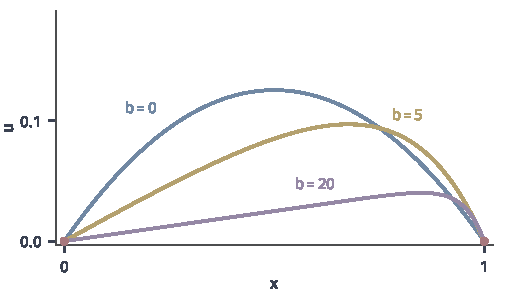
\includegraphics[width=86mm]{figures/06-differential-equations/02-partial-differential-equations/matplotlib/ellip-nonsymmetric/figure.pdf}
  \caption{非对称问题$-u''+bu'=1$的解随$b$的变化。$b=0$（蓝）时对称，$b=5$（黄）与$b=20$（紫）时被对流推向右端，在$x=1$附近形成边界层。双线性型的二次部分与$b$无关，所以这些解不能由式~\eqref{eq:ellip-energy}的极小化得到。}
  \label{fig:ellip-nonsymmetric}
\end{BookInlineFigure}

区间上的这个例子还可以用积分因子补救。在方程两边乘以$\mathrm{e}^{-bx}$，得到$-(\mathrm{e}^{-bx}u')'=\mathrm{e}^{-bx}f$，它在带权的能量下又是对称的。多维情形中，只有当一阶项的系数是某个函数的梯度时，这种办法才能奏效，否则一般不存在把问题化成能量极小的权函数。所以结论是：Lax--Milgram定理适用的范围比能量极小更广，能量极小只是对称情形的额外结构。
